%%-------------------------------------------------- READ THE COMMENTS CAREFULLY ------------------------------------------%%
%%%%%%%%%%%%%%% Template for generating Report and Presentation according to G.N.D.E.C., Ludhiana's format %%%%%%%%%%%%%%%%%%%%%%%
%% Here myclass is the class name
%% print is used for making a report
%% screen is used for making a presentation
%% If you want the content common in print and screen, then don't specify the content in screen or print environment.
%%----------------------------------------------------------------------------------------------------------------------------
\documentclass[12pt]{priclass}
\usepackage[sectionbreak]{pdfscreen}             %% If you want to produce presesntation then use screen, otherwise use print
%---------------------------------------------------
\usepackage{setspace}
\linespread{1.5}
\usepackage{float}

\renewcommand{\rmdefault}{ptm}				%% font style Times New Roman
\usepackage{titlesec}
\titleformat{\chapter}[display]
    {\normalfont\huge\bfseries}{\chaptertitlename\ \thechapter}{20pt}{\Huge}
\titlespacing*{\chapter}{0pt}{-35pt}{30pt}
%----------------------------------------------------
%%%%%%%%%%%%%%%%%%%% Page Setting %%%%%%%%%%%%%%%%%%%%%%%%%%%

                        %% Here replace your project name
\usepackage[left=2.5cm, right=1.5cm, top=2.5cm, bottom=1.5cm]{geometry}
%\pagestyle{fancy}

%-----------------------------------------%% These commands are used in first page after titlepage
\newcommand{\student}{\vskip 2.5cm}
\newcommand{\supervisor}{\vskip 2cm}
\newcommand{\stamp}{\vskip 2.5cm}                                
%%%%%%%%%%%%%%%%%%%%%%%%%%%%%%%%%%%%%%%%%%%%%%%%%%%%%%%%%%%%%%%%%%%%

%%%%%%%%%%%%%%%%%%%%% Title page %%%%%%%%%%%%%%%%%%%%%%%%%

\uppercase{ \title{e-Notice Application}}
\subtitle{For Android Phones}
\purpose{REPORT} % or synopsis or Mid term report
\branch{IT} 

\author{Priyanka Kapoor}
\classrollno{106160}
\unirollno{100371180720}

\name{Submitted to which guide} %Prof. Sukhjit Singh Sehra

\branch{Information Technology}     %%INFORMATION TECHNOLOGY


%%----------------------------------------------------------------------%%




%%%%%%%%%%%%%%%%%%%%%%%%%%%%%%%%%%%%%%%%%%%%%%%%%%%%%%%%%%%%%%%%%%%%%%

%%------------------- Body of document----------------------------------%%
\begin{document}


 \maketitle                                 %%% Title page for report


\pagenumbering{Roman}                  %% Pagenumering can be in Roman or arabic
%\cfoot{\thepage}                     %% cfoot means centered footer(page no.)

%-------------------------------------------------------------------
\begin{center}
\textbf{Abstract}                           %% '*' is used to unnumbered the section
\end{center}
e-Notice App helps you access online notices on your phone. It is an online notice board maker
where a group of people can easily communicate with each other by sticking virtual notes. These
notes can have text, images or include online videos such as from YouTube.\\ \\
The notice board has always been the place where staff/students gathers to get their latest release
of corporate news. eNotice brings the notice board to a virtual location where staff/students can
not only read notices, but immediately react and respond to them - from their own desks!
With this electronic notice and announcement system, notification may be sent out notifying
staff that a new notice has been posted, where staff may know if it concerns him directly.\\ \\
In this way, e-Notice Application also serves as a mailing list for all employees in the directory. This eliminates the
need to keep a separate mailing list which is hard to maintain due to the rapid movement of staff.


%---------------------------------------------------------------------------

\begin{center}
\textbf{Acknowledgment}                           %% '*' is used to unnumbered the section
\end{center}
The author is highly grateful to the Dr. M.S. Saini (Director, Guru Nanak Dev Engineering College, Ludhiana) for providing this opportunity to carry out the six month training at Testing and Consultancy Cell, Guru Nanak Dev Engineering College, Ludhiana.\\
 The constant guidance and encouragement received from Er. K. S. Mann (Dean Training and Placement Cell, Guru Nanak Dev Engineering
College, Ludhiana) has been of great help in carrying out the project work and is acknowledged with reverential thanks.\\
 The author would like to express a deep sense of gratitude and thanks profusely to Mr. Sachin Khosla (CEO, DigiMantra Labs,
IT Park, Ludhiana). Without their wise counsel and able guidance, it would have been impossible to complete the report in this manner. \\
The help rendered by Mr. Rustam Singh, Associate Software Developer (DigiMantra Labs, Ludhiana) for experimentation is greatly acknowledged.\\
The author express gratitude to other faculty members of Information Technology department of Guru Nanak Dev Engineering College for their intellectual support throughout the course of this work.\\ \\
Finally, I am indebted to all whosoever have contributed in this report work and friendly stay at DigiMantra Labs, Ludhiana.\\ \\
\textbf{Priyanka Kapoor}

%%At last specify the co-helpers.

%----------------------------------------------------------------------------------------
%---------------------------------------------------------
%\section*{To Whom it may concern}                        %% '*' is used to unnumbered the section
I here by certify that Your Name Roll No.   of Guru Nanak Dev Engineering College Ludhiana, has undergone six months/weeks training from starting date to end date at our organisation to fulfil the requirements for the award of degree of B.Tech (year and branch). He works on {project name} project during the training under the supervision of (Mentor name). During his tenure with us we found him sincere and hard working. Wishing him a great success in the future.
\student
Signature of the Student
\supervisor
Signature of the Supervisor 
\stamp
(Seal of Organisation)

%---------------------------------------------------------------




\tableofcontents 
\newpage       %% This command automatically generates Index page
\listoffigures                         %% This command creates a list of figures in the document
\newpage
%\thispagestyle{empty}

\pagenumbering{arabic}                  %% now onwards arabic page numbeing is required
 %\cfoot{\thepage}                       %% centered footer (page no.)

%------------------------------------------------------
\chapter{Introduction}
\section{Introduction To Organisation}
I had my six months industrial training at DigiMantra Labs, IT Park, Ludhiana.
DigiMantra Labs is an IT company based in India. It was established in 2009. The CEO of this company is Mr. Sachin Khosla. DigiMantra mainly focus in development of preeminent Web, Mobile and Desktop solutions. It believes  in delivering quality and cater diversified niche of industries. DigiMantra have a proven track record of delivering high performance solutions to various big to small level industries. This company is aided by Government of India.\\\\
DigiMantra Labs is a customary participant of various important events like IndiaSoft, ICT – HongKong. It always look forward to build new relationships with like minded companies/ individuals. 
DigiMantra has a  team of young dynamic professionals formed by the group of engineers who have graduated from reputed Engineering Colleges. Their team is lead by professional who has worked with big products like Limewire, Trulia etc. 
\\\\
Good thing about DigiMantra is that it is driven by ethical values, energy to build great apps and determination to deliver the best. They are keen to provide out of box solutions to the client keeping the ‘cost to company’ aside.
 DigiMantra teams are trained to work under various software models such as Agile, Scrum etc. They make sure that they adhere to these standards so that they are able to deliver quality product 
 All the activities at office are closely monitored and recorded using CCTV cameras. We just ensure that your business plan is safe with us.
DigiMantra innovate and build our applications using latest technologies, which makes them fast, robust \& scalable. This company contributes to open source software by organizing / participating in OSS Camps.\\
Their expertise is in the following fields:-\\
\begin{itemize}
\item Enterprise Level Product Development 
\item Internet Tools including Viral campaigns, Affiliate Marketing solutions 
\item Mobile Application Development; iOS \& Android 
\item Cloud Computing Solutions – SaaS \& PaaS 
\item Website Development with Complete CMS and Social Networking Support 
\item User Experience \& Product Designing 
\item Social Media Applications \& Campaigning 
 \end{itemize}
\begin{figure}[h]
\centering 
\includegraphics[scale=0.9]{image/digimantra.png}
\caption[GNDEC]{DigiMantra Labs Logo}
\end{figure}
DigiMantra believes that 'communication' is the foremost ingredient to make a project successful. It communicate with the clients on regular basis and using the dedicated VOIP lines and various other ways of communication. 
This company understand different needs of different customers and hence have custom solutions based on the requirement. Their onsite team facilitation is one such example.

%%%%%%%%%%%%%%%%%%%%%%%%%%%%%%%%%%%%%%%%%%%%%%%%%%%%%%%%%%%%%%%%%%%%%%%%%%%%%%%%%%%%%%%%%%%%%%%%%%%%%%%%%%%%%%%%%%%%%%%%%%%%%%%%%%%
\pagebreak
\section{Introduction to Project}

e-Notice App helps you access online notices on your phone. It is an online notice board maker
where a group of people can easily communicate with each other by sticking virtual notes. These
notes can have text, images or include online videos such as from YouTube.\\\\
The notice board has always been the place where staff/students gathers to get their latest release
of corporate news. eNotice brings the notice board to a virtual location where staff/students can
not only read notices, but immediately react and respond to them - from their own desks!
With this electronic notice and announcement system, notification alerts may be sent out notifying
staff and students that a new notice has been posted, where staff may know if it concerns him directly. In this
way, e-Notice also serves as a mailing list for all employees in the directory. This eliminates the
need to keep a separate mailing list which is hard to maintain due to the rapid movement of staff.\\ \\
These are the features that an eNotice App should have:
\begin{itemize}
\item An electronic dashboard board for disseminating information out to staff and students.
\item Notices can be posted, with response obtained instantly.
\item Staff or student can be notified of new postings via notification alert.
\item Notice administrator may push important notices in to selected staff's email.
\item Notice administrator may create any notice category.
\end{itemize}
The interface of this application is straightforward and takes you roughly a minute to get started.
Adding notes to board is easy, just click on the post notice button and enter the text. Users can view the post 
on the spot by having a notification alert in android phone.
Here registration is must for all the users having this application in order they want to have notification and staying stuned.\\ \\
This application can also acts as a market place and lets you advertise, for example, a room to
rent, a car for sale, a job opportunity, a house for sale, an upcoming event, an announcement, a
service, and so on.
\\
This application creates interactive notice boards online. You can customize boards with a
custom background, title and background images. It allows users to add sticky notes with text,
images and videos. You can set preferences on who can edit and view the board. Facility of drag
and drop notes anywhere on the board is available. Users can sign using their Google accounts /
Facebook Account and can share boards with others.

%%%%%%%%%%%%%%%%%%%%%%%%%%%%%%%%%%%%%%%%%%%%%%%%%%%%%%%%%%%%%%%%%%%%%%%%%%%%%%%%%%%%%%%%%%%%%%%%%%%%%%%%%%%%%%%%%%%%%%%%%%%%%%%%%%%
\pagebreak
\section{Project Category (Mobile Application) }

"e-Notice App" is a mobile application i.e an Internet based Mobile application. A mobile application is a computer program designed to run on smartphones, tablet computers and other mobile devices.
Apps are usually available through application distribution platforms, which began appearing in 2008 and are typically operated by the owner of the mobile operating system, such as the Apple App Store, Google Play, Windows Phone Store, and BlackBerry App World.\\\\
Mobile apps were originally offered for general productivity and information retrieval, including email, calendar, contacts, and stock market and weather information. However, public demand and the availability of developer tools drove rapid expansion into other categories, such as mobile games, factory automation, GPS and location-based services, banking, order-tracking, ticket purchases and recently mobile medical apps. The explosion in number and variety of apps made discovery a challenge, which in turn led to the creation of a wide range of review, recommendation, and curation sources, including blogs, magazines, and dedicated online app-discovery services.
\\ \\
Mobile application development is the process by which application software is developed for low-power handheld devices, such as personal digital assistants, enterprise digital assistants or mobile phones. These applications can be pre-installed on phones during manufacturing, downloaded by customers from various mobile software distribution platforms, or delivered as web applications using server-side or client-side processing (e.g. JavaScript) to provide an "application-like" experience within a Web browser.\\ \\
 Application software developers also have to consider a lengthy array of screen sizes, hardware specifications and configurations because of intense competition in mobile software and changes within each of the platforms. Mobile app development has been steadily growing, both in terms of revenues and jobs created. 
The popularity of mobile apps has continued to rise, as their usage has become increasingly prevalent across mobile phone users.

%%%%%%%%%%%%%%%%%%%%%%%%%%%%%%%%%%%%%%%%%%%%%%%%%%%%%%%%%%%%%%%%%%%%%%%%%%%%%%%%%%%%%%%%%%%%%%%%%%%%%%%%%%%%%%%%%%%%%%%%%%%%%%
\pagebreak
\section{Objective}

The proposed system's objectives are to overcome all the limitations and drawbacks of the
existing system. The online ‘eNotice’ application is user-friendly android application. The main
objective of the application is its simplicity of design and ease of implementation that shows and
helps to collect most of the information about events going on in college premises. The interface
will be very user-friendly. \\ \\
The main objectives of the proposed system can be enumerated as follows:
\begin{itemize}
\item Faster dissemination of notices regarding education, technical events, cultural events.
\item Any lost/found going out in college.
\item Easy way to broadcast your message.
\item Helps you to be updated with whats going on in College.
\item Good way to advertise about Tuitions/ Coaching and Courses.
\item User can also follow a group notice board.
\end{itemize}

%%%%%%%%%%%%%%%%%%%%%%%%%%%%%%%%%%%%%%%%%%%%%%%%%%%%%%%%%%%%%%%%%%%%%%%%%%%%%%%%%%%%%%%%%%%%%%%%%%%%%%%%%%%%%%%%%%%%%%%%%%%%%%%
\pagebreak
\section{Problem Formulation}

To develop a mobile application that will help you receiving the notices from the college, anywhere , anytime. Earlier their was problem that notices were pasted on notice board. If there is holiday on the next day, nobody will be able to read it. Moreover any update on website is also very difficult. Everyone feels lazy to go and update the website data. The more easy way is, just type in message sitting wherever and post by pressing a button. It will notify all the staff and students, registered with that application. \\

%%%%%%%%%%%%%%%%%%%%%%%%%%%%%%%%%%%%%%%%%%%%%%%%%%%%%%%%%%%%%%%%%%%%%%%%%%%%%%%%%%%%%%%%%%%%%%%%%%%%%%%%%%%%%%%%%%%%%%%%%%%%%%%%%
\pagebreak
\section{Identification of Need}
\begin{enumerate}
\item As we discussed earlier that manual maintenance of a notices is a tedious
job. So to enhance the ease of working, we go for this package.

\item Giving  the facility to convey messages to all students anytime and anywhere.

\item Making students updated about all the events and activities going on in the college.

\item The student will not require to stand in the crowd to see the notice.
There wil be no issue of fighting in order to see the notice first. Everyone is first to see that notice inside thier own mobile phone 
anywhere and anytime.
\item The least but most important it saves time.

\item Utilizing less man power. As there are many persons involved in circulating the message. With this application, only one person is required to post the notice. Rest of the man power is saved in the entire process.

\end{enumerate}

%%%%%%%%%%%%%%%%%%%%%%%%%%%%%%%%%%%%%%%%%%%%%%%%%%%%%%%%%%%%%%%%%%%%%%%%%%%%%%%%%%%%%%%%%%%%%%%%%%%%%%%%%%%%%%%%%%%%%%%%%%
\pagebreak
\section{Existing System}
Currently our college has manual system of putting notices on notice board. Its outdated now.
As nobody has a time to stand in rush in order to read the notices on noticeboard.

\textbf{\emph{Limitations of Existing System:}}
\begin{enumerate}
\item \textbf{\emph{Order of Data}}: Notice can get out of order in traditional notice board system. If
someone accidentally puts some data in the wrong place, it can lead to lost data. Automated
notice management systems allow users to quickly check whether information already exists
somewhere in the system, which helps avoid problems like redundant data.
\item \textbf{\emph{Complexity}}: Automated system is less complex than manual system of handling notices, which can make
it easier for untrained people to access and manipulate data. Anyone having the basic knowledge
of mobiles can work on the automated system.
\item \textbf{\emph{Inconsistency of data}}: There will be an unavailability for future use, since notice might get
misplaced during manual notices management. So notice won't be preserved properly for future
use.
\item \textbf{\emph{Damage}}: Manual notices stack are vulnerable to damage, destruction and theft in ways that digital
databases are not. A company may back up its digital data both on site and at offsite locations,
ensuring its security if the office building suffered a fire or similar disaster. A manual database,
however, may only exist in one place without any copies.
As a result, a manual database would be very vulnerable to a fire or other natural disaster. In
addition, while access time in a manual database system, information must be found by hand
rather than electronically. While a digital database will typically allow users to search the entire
database for specific information in seconds, someone looking for information in a manual system
may have to spend hours searching for a particular piece of data.
\item \textbf{\emph{Editing and Communication}}: Manual notices do not allow users to easily edit data or
information. Manual notices often cannot be edited directly, forcing users to make new copies.
To circulate notice on paper, users must require peons and other staff. e-Notice app allow
users to edit information fields directly, and because data is stored digitally, it is already in a form
that can be easily transmitted.
\end{enumerate}
%%%%%%%%%%%%%%%%%%%%%%%%%%%%%%%%%%%%%%%%%%%%%%%%%%%%%%%%%%%%%%%%%%%%%%%%%%%%%%%%%%%%%%%%%%%%%%%%%%%%%%%%%%%%%%%%%%%%%%%%%%%%%%%%

\pagebreak
\section{Proposed System}
Proposed System will be able to do the following:
\begin{enumerate}
\item \textbf{\emph{To eliminate wastage of time and energy:}}\\
e-Notice app will be able to save lot of paper and time. It directs both teacher and pupils’ energy and attention to one
thing at a time by placing proper persons at their proper places at the proper time. Everything will be instanteneous.
\item \textbf{\emph{To avoid duplication and overlapping:}}\\
This application will help to remove the duplicacy of notices. Only one person, who is admin can post the notice.
No one else would be able to do so. Soo student and staff will be given correct information all the time.
\item \textbf{\emph{To ensure due attention of student to each and every notice:}}\\
e-Notice App ensures that everyone has kind attention to every notice and updates going on in college.
There will be a buzz at each and every notice to drive the attention of student to check it once.
In this way, students will be well informed about their college activities.
\item \textbf{\emph{To bring system into college life:}}\\ 
It would be dire need of all colleges as its easy and shortcut method to inform all the students. In the absence of proper notification system will make it very difficult to inform students at right time.
\item \textbf{\emph{Searching a particular Notice:}}\\
This application allows you search the notice very easily through title of notice. If anyone forgots about the
notice details, he can search it out very easily.

\item \textbf{\emph{Free Service:}}\\
It gives free service to notify all the students. There will be no cost of sending notification to all.
Just have the good system implemented in college and that too free of cost.

\item \textbf{\emph{Prevent Crowd in College:}}\\
As you can see, there is always a crowd at notice board. As notice board is one, and people to see notice are more.
With this application there will be no more crowd. Everyone will be well informed even at their homes. So they are
free to do there other work.

\item \textbf{\emph{Automatically Updated Dashboard:}}\\
The dashboard of notice is automatically updated when a new message arrives. The user can himself refreah the dashboard 
to see any new notice.

\item \textbf{\emph{Anytime Anywhere Service:}}\\
With this application, notices will be delivered anytime and at any place. There is no restriction of time to 
send a notice.

\item \textbf{\emph{Keeping Notices at one place:}}\\
This application allow you to have notices in one place only. If there is an attachment with that, all will be placed in a separate
folder dedicated to that aplication. So there will be no here and there of notices.
\end{enumerate} 

%%%%%%%%%%%%%%%%%%%%%%%%%%%%%%%%%%%%%%%%%%%%%%%%%%%%%%%%%%%%%%%%%%%%%%%%%%%%%%%%%%%%%%%%%%%%%%%%%%%%%%%%%%%%%%%%%%%%%%%%%%%%%%%%%%%%
\pagebreak
\section{Unique Features of System}
The unique features of this application are as follow:
\begin{enumerate}
\item \textbf{\emph{GCM Notification}}:
Google Cloud Messaging has been used to broadcast notices to all the students who are registered with this application. It will help you 
receive the notice even if you application is closed. So it implements anywhere anytime notifications.Google Cloud Messaging (GCM) is a free service for sending messages to Android devices. GCM messaging can greatly enhance the user experience. Your application can stay up to date without wasting battery power on waking up the radio and polling the server when there are no updates. Also, GCM allows you to attach up to 1,000 recipients to a single message, letting you easily contact large user bases quickly when appropriate, while minimizing the work load on your server.

\item \textbf{\emph{Battery Saving Application:}}\\
This application saves your battery too. Its because, the service implemented in application is not running all the time. Whenever GCM ping 
the mobile, only then it makes a broadcast to phone that initiates the service. In this way, its saving your battery alot.

\item \textbf{\emph{Automatically Updated Dashboard:}}\\
The dashboard of notice is automatically updated when a new message arrives. The user can himself refreah the dashboard 
to see any new notice.

\item \textbf{\emph{Anytime Anywhere Service:}}\\
With this application, notices will be delivered anytime and at any place. There is no restriction of time to 
send a notice.

\item \textbf{\emph{Keeping Notices at one place:}}\\
This application allow you to have notices in one place only. If there is an attachment with that, all will be placed in a separate
folder dedicated to that aplication. So there will be no here and there of notices.

\item \textbf{\emph{Free Service:}}\\
It gives free service to notify all the students. There will be no cost of sending notification to all.
Just have the good system implemented in college and that too free of cost.

\item \textbf{\emph{Case Pictures in One Folder:}}\\
The attachments of notices goes at one place only. If you want to see all attachments, you can go in gallery and can see it. 
Its a good feature of this application that cares for our files organisation in phone too.
\end{enumerate}


%-----------------------------------------------------------
\chapter{Requirement Analysis and System Specifications}
\section{Feasibility Study}
Depending on the results of the initial investigation, the survey is expanded to a
more detailed feasibility study. Feasibility study is a test of system proposal ac-
cording to its work ability, impact on the organization, ability to meet user needs,
and effective use of resources. The objective for this phase is not to solve the
problem but to acquire a sense of scope. During the study, the problem definition
is crystallized and aspects of the problem to be included in the system are deter-
mined.\\ \\
Mobile Application Development Systems are capital investments because resources
are being spent currently in order to achieve benefits to be received over a pe-
riod of time following completion. There should be a careful assessment of each
project before it is begun in terms of economic justification, technical feasibility,
operational impact and adherence to the master development plan.
We started the project by listing the possible queries that the user might want
to be satisfied. And on these lines we guided the project further.\\ \\
The three main points, kept in mind at the time of project, are :
\begin{itemize}
\item Possible (To build it with the given technology and resources)
\item Affordable (given the time and cost constraints of the organization)
\item Acceptable (for use by the eventual users of the system
\end{itemize}

The three major areas to be considered while determining the feasibility of a
project are :
\begin{enumerate}
\item \textbf{\emph{Technical Feasibility:}} The technical issue usually raised during the feasi-
bility stage of the investigation includes the following :
\begin{itemize}
\item Does the necessary technology exist to do what is suggested?
\item Do the proposed equipments have the technical capacity to hold the
data required to use the new system?
\item Will the proposed system provide adequate response to inquiries, re-
gardless of the number or location of users?
\item Can the system be upgraded if developed?
\item Are there technical guarantees of accuracy, reliability, ease of access
and data security?
\end{itemize}

Earlier no system existed to cater to the needs of ’Secure Infrastructure Im-
plementation System. The current system developed is technically feasible.
It is a web based user interface. Thus it provides an easy access to the
users. The databases purpose is to create, establish and maintain a work-
flow among various entities in order to facilitate all concerned users in their
various capacities or roles. Permission to the users would be granted based
on the roles specified.
Therefore, it provides the technical guarantee of accuracy, reliability and
security. The software and hardware requirements for the development of
this project are not many and are already available as free as open source.
The work for the project is done with the current equipment and existing
software technology. Necessary bandwidth exists for providing a fast feed-
back to the users irrespective of the number of users using the system.

\item \textbf{\emph{Operational Feasibility:}} Under this category of service we conduct a study to analysis and determine whether your need can be fulfilled by using a proposed solution. The result of our operational feasibility Study will clearly outline that the solution proposed for your business is operationally workable and conveniently solves your problems under consideration after the proposal is implemented. We would precisely describe how the system will interact with the systems and persons around. Our feasibility report would provide results of interest to all stakeholders. It will do as per the needs of the business requirements.

\item \textbf{\emph{Timeline Feasibility:}} It is important to understand that a need must be fulfilled when it has to be. Some otherwise feasible and highly desirable projects can become non-feasible due to very restrictive timeline constraints. This fact makes it imperative that milestones are clearly linked to the timeline and projects are well conceived with safe unforeseen margins. We make sure that we strictly follow what has been stated above.

\end{enumerate}

\pagebreak

\section{Software Requirement Specification Document}

\subsection{Data Requirements}
Data requirement is meant to be the data that will be used in our application. Data required in this project is all notices, that need to be conveyed to the user. This application also require the username and passwords of persons in order to register them and sending notification about updates. So two main requirements are:
\begin{itemize}
\item {Notice Details}
\item {User Details}
\end{itemize}

\subsection{Functional Requirements}
In order to make this application functional, we require the following:
\begin{itemize}
\item \textbf{\emph{Download mobile application:}}\\
A user should be able to download the mobile an
application through either an application store or
similar service on the mobile phone. The application should be free to download.
\item \textbf{\emph{User registration:}}\\
Given that a user has downloaded the mobile application, then the user should be able to register
through the mobile application. The user must provide user-name, password and e-mail address. The user 
can choose to provide a regularly used phone number.

\item \textbf{\emph{User Login:}}\\
Given that a user has registered, then the user should be able to log in to the mobile application.
The log-in information will be stored on the phone and in the future the user should be logged in automatically. 

\item \textbf{\emph{Reset Password:}}\\
Given that a user has registered, then the user should be able to retrieve his/her password by e-mail. 

\item \textbf{\emph{DashBoard:}}\\
Given that a user is logged in to the mobile application, then the first page that is shown should be
the dashboard page. The user should be able to see all the college notices.

\item \textbf{\emph{Search Notice:}}\\
The user should be able to search for a notice by its title. For example, if a user types fee, all the notices having fee in their content get displayed.

\item \textbf{\emph{Selecting a Notice:}}\\
 A user should be able to select any notice from list view. The click on particular notice will take him to notice details
 of that particular notice.

\item \textbf{\emph{Navigating back to Notices List:}}\\
The user should be able to navigate back to notices list from the notice details section. This is required to give a 
good user experience.

\item \textbf{\emph{Deleting Notices:}}\\
The user should have the option to delete the unnecessary notices from his phone, by ticking them one by one and then deleting them in one go. This way, user can save this phone memory from unrequired notices.

\item \textbf{\emph{Posting Notices:}}\\
The admin of this application should be able to post the notices. He should be able to add a picture within notices. That picture
can be taken either from gallery or by using the camera of the mobile phone.

\item \textbf{\emph{Notification Alert:}}\\
All the registered users should be able to have a ping or notification on their mobile phone whenever a new notice is posted.

\end{itemize}

\subsection{Performance Requirements}
The requirements in this section provide a detailed specification of the user interaction with the software and measurements placed on the system performance.
\begin{itemize}
\item \textbf{\emph{Prominent search feature:}}\\
The search feature should be prominent and easy to find for the user.

\item \textbf{\emph{Usage of the Notice Information:}}\\
The notice link should be prominent and it should be evident that it is a usable link.
Selecting the notice link should only take one click.

\item \textbf{\emph{Response Time:}}\\
The reponse time should not be more than 5 seconds if user have a proper internet connection. 

\item \textbf{\emph{Fault Tolerance:}}\\
The fault tolerance of the system should be very good. If the system loses the connection to the Internet or the system gets some 
strange input, the user should be informed.

\end{itemize}

\subsection{System Dependability}
Following are the requirements that an application require from the device/mobile on which it is installed.
\begin{itemize}
\item \textbf{\emph{Internet Permission:}}\\
Application develeped, require full internet permissions of mobile so that it can fetch notices from the server.
At the same time, it should be able to receive buzz or notification tone whenever new notice is posted by admin.

\item \textbf{\emph{External SD Card Writable Permissions:}}\\
This application would be requiring read write access to SD card. It is required in order to download the notices attachment and save
in SD card of mobile phone.

\item \textbf{\emph{System Tools:}}\\
This application require various system tools to be used. For example, it requires Camera of mobile in order to click the image and
post in into notice. It also require system tool, that prevents it from sleeping.

\item \textbf{\emph{Hardware Control:}}\\
It uses vibrator of mobile phone whenever any notification arrives.

\item \textbf{\emph{Account Info:}}\\
It also fetches your google account information in order to get the user registered with Google Cloud Messaging.
\end{itemize}

\subsection{Maintainability Requirements}
Following are the maintainability requirement of e-Notice mobile application:
\begin{itemize}

\item \textbf{\emph{Application extendibility:}}\\
The application should be easy to extend. The code should be written in a way that it favors
implementation of new functions. It is requires in order for future functions to be implemented easily to the application.

\item \textbf{\emph{Application testability:}}\\
Test environments should be built for the application to allow testing of the applications different
functions.

\end{itemize}

\subsection{Security Requirements}
\begin{itemize}
\item \textbf{\emph{Communication Security:}}\\
There shoulb be security of the communication between the system and server.The messages should be
 encrypted for log-in communications, so others cannot get user-name and password from those messages.
Every exchanged of information between client and server should be encrypted so that no one can track it.
\item \textbf{\emph{Admin Login Account Security:}}\\
If an admin tries to log in to the web portal with a non-existing account then the admin should
not be logged in. The admin should be notified about log-in failure.
\item \textbf{\emph{Admin Account Security:}}\\
There should be security of admin accounts. An admin and IP address should not be able to log-in to the web portal for a certain time period
after three times of failed log-in attempts.

\item \textbf{\emph{User Create Account Security:}}\\
The security of creating account for users of the system should be maintained. If a user wants to
 create an account and the desired user name is occupied, the user should be asked to choose a different user name.
\end{itemize}
\subsection{Look and Feel Requirements}

Regarding look and feel, our client is straight forword. They believe in simplicity. So these are their requirements:
\begin{itemize}
\item \textbf{\emph{Simple and Light:}}\\
The user interface should be simple and lightly colored. It should give relaxing effect on looking at its GUI. No bright
colors should be used while designing the UI of this application.

\item \textbf{\emph{Easy to Use}}\\
The application should be easy to use. If any user is doing something wrong, he/she should be informed correctly, what is going
wrong behind the scene. There should be proper instructions for the user to use this application.

\item \textbf{\emph{Soft Sound Notification:}}\\
The sound for notification should be very soft. It should not distrub the pers with a loud note.
Everything should be sober in this application.
\end{itemize}

%%%%%%%%%%%%%%%%%%%%%%%%%%%%%%%%%%%%%%%%%%%%%%%%%%%%%%%%%%%%%%%%%%%%%%%%%%%%%%%%%%%%%%%%%%%%%%%%%%%%%%%%%%%%%%%%%%%%%%%%%%%%%%%%
\pagebreak
\section{Validations}
Any application is useless without validation. There should be a way to validate the user input first before sending the user request to the server. Following are the validations implemented in proposed system:
\begin{itemize}
\item \textbf{\emph{User Password Validation:}}\\
The application should check the user and password fields before sending any request to the server. It should check whether the fields are
filled or not. if fields are not filled up, user should be instructed to fill up the fields before moving further. in this way, there will
be less traffic on the server.

\item \textbf{\emph{Validations During Registration:}}\\
There are a lot of validations that needs to be implemented in the application. They are as follow:
\begin{enumerate}

\item \textbf{\emph{First and Last Name of User:}}\\
The first and last name of user should be not null. Also first letter of first and last name should be in uppercase.

\item \textbf{\emph{Username:}}\\
The username can contain only alphabets, digits, underscore and hyphen. It should be atleast 3 characters long and maximum of 15 characters.

\item \textbf{\emph{Password:}}\\
The password must contains one digit from 0-9, one lowercase character,one uppercase character, one special symbols in the list "\@\#\$\%" and length of password must be at least 6 characters and maximum of 20.

\item \textbf{\emph{Email:}}\\
The application must validate and email address entered by the user before sending request to the server.

\item \textbf{\emph{Mobile Number:}}\\
The mobile number should be of only ten digits. No more, no less than that.
\end{enumerate}

\item \textbf{\emph{Validating During Posting Notices:}}\\
The application should validate the notice posting fields before posting any notice. It should check whether title and description fields are filled or not. if not, it should tell the user to fill up the required fields while posting the notice.

\item \textbf{\emph{Reset Password Validation:}}\\
The application should check that user has entered the username or email in the given filed before pressing the reset password button.

\end{itemize}

%%%%%%%%%%%%%%%%%%%%%%%%%%%%%%%%%%%%%%%%%%%%%%%%%%%%%%%%%%%%%%%%%%%%%%%%%%%%%%%%%%%%%%%%%%%%%%%%%%%%%%%%%%%%%%%%%%%%%%%%%%%%%%%%%%%%
\pagebreak
\section{Expected Hurdles}
The main hurdles that can come in the notice are as follow:
\begin{enumerate}
\item \textbf{\emph{GCM Notification:}}\\
Its possible that there may be a problem with receiving GCM notifications. When to receive a broadcast signal and when to start the service.
If service is not started at the proper time, there may be the case, user will not be able to receive any notification from the server.

\item \textbf{\emph{Device Database:}}\\
Its very much difficut to see entries going inside the device database. You have to check through coding. You can't access the applications database easily. So its bit hard to debug the database errors.

\item \textbf{\emph{Device SD Card:}}\\
The application will be requiring access to the SD card of the user mobile. It may be possible that SD Card is full or missing SD Card. So the user will not be able to receive the respective attachment of notices.

\item \textbf{\emph{Google Play Services:}}\\
Registering to the GCM Server requires to have Google Play services on device installed. Otherwise user will not be able to register 
to GCM server nor will be able to receive any message.
\end{enumerate}

%%%%%%%%%%%%%%%%%%%%%%%
\pagebreak
\section{SDLC Model Used}
This section describes the project as per the various stages of the Software Development life
cycle. The model of software development life cycle used in this project is the waterfall method.
The Waterfall Method is comprised of a series of very definite phases, each one run intended to
be started sequentially only after the last has been completed, with one or more tangible
deliverables produced at the end of each phase of the waterfall method of SDLC. Essentially, it
starts with a heavy, documented, requirements-planning phase that outlines all the requirements
for the project, followed by sequential phases of design, coding, test-casing, optional
documentation, verification (alpha-testing), validation (beta-testing), and finally
deployment/release.\\


\begin{figure}[H]
\centering 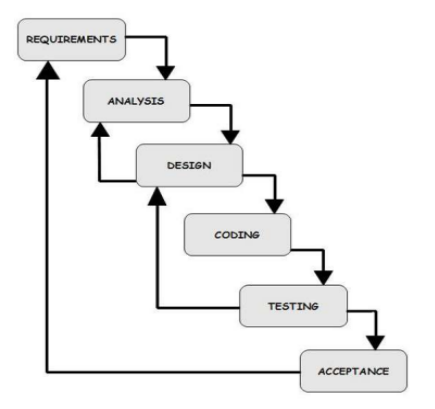
\includegraphics[scale=0.7]{image/sdlc.png}
\caption{Login Page}
\end{figure}
\begin{enumerate}
\item \textbf{\emph{Requirement Analysis:}}\\
Existing system is time consuming and it makes difficult to convey huge amount of users about
any event, class or seminar almost instantly. Also there is always a big crowd in front of
noticeboard. So it was hectic to read any useful instruction and information. Thus all the
problems of the existing system are summarized and proposing a new system that works as an
online application. It is a value added solution to the problem. It resolves all the problems stated
above. It will provide simple interface to the user to operate on and convey the intended users
about events almost instantly, anytime and anywhere.
\item \textbf{\emph{Design:}}\\
It includes translation of the requirements specified in the SRS into a logical structure that can be implemented in a programming language. The output of the design phase is a design document that acts as an input for all the subsequent SDLC phases. The design of this app is simple and user friendly containing six main activities, namely:
\begin{enumerate}
\item Register 
\item Login
\item Dashboard
\item Details of Notices
\item Admin Panel 
\item Reset Password
\end{enumerate}

\item \textbf{\emph{Coding/Implementation:}}\\
It includes translation of the requirements specified in the SRS into a logical structure that can be implemented in a programming language. The output of the design phase is a design document that acts as an input for all the subsequent SDLC phases. The project is implemented using the Android virtual devise (AVD). This emulator helped to implement the project in a real-like environment and sketch out the details of how it will work on a real hardware. Each activity is linked with another and interconnectivity is transparent and smooth.

\item \textbf{\emph{Testing:}}\\
It includes detection of errors in the application. The testing process starts with a test plan that recognizes test-related activities, such as test case generation, testing criteria, and resource allocation for testing. The code is tested and mapped against the design document created in the design phase. The output of the testing phase is a test report containing errors that occurred while testing the application. Testing of the project has not been done on  real hardware and also on the emulator or software environment. Testing has been done for each of the individual activities of the project.

\item \textbf{\emph{Maintenance:}}\\
It includes implementation of changes that software might undergo over a period of time, or implementation of new requirements after the software is deployed at the customer location. The maintenance phase also includes handling the residual errors that may exist in the software even after the testing phase. The project maintenance is low cost and efficient as user will get this application at free of cost and also this application is shared over network, therefore maintenance is little bit difficult. 

\end{enumerate}

%-------------------------------------------------
\chapter{System Design}

\section{Design Approach}
A design approach is a general philosophy that may or may not include a guide for specific methods. Some are to guide the overall goal of the design. Other approaches are to guide the tendencies of the designer. A combination of approaches may be used if they don't conflict.\\
\emph{Function Oriented Design Approach:}\\
Function Oriented Design Approach is partitioning of a design into subsystems and modules, with each one handling one or more functions. Contrast with object-oriented design, data-structure-oriented design. \\

This application project uses function oriented design approach. Every module and sub modules are made, based on their functionality.
These modules are designed and implemented separately and then they are integrated together to form the desired application.

\section{Detail Design}
The detailed design of this application is as follow:
\begin{enumerate}
\item \textbf{\emph{Registering a User:}}\\
The first step in this application is to get the users registered to both GCM Server and to Remote Web Server. For this, user will provide all the necessary details and press the register button. The request will first go to Google Cloud Messaging Server. GCM Server will provide
the registration id for that device. After that, all the information along with registration id is stored on Web Server and the user gets registered.

\item \textbf{\emph{User Login:}}\\
After registering, the user is allowed to log in. Username and password after validating at client side, is sent to server side to authentication. After authentication response is sent by the server to client, and then user gets logged in.

\item \textbf{\emph{Viewing the Notices:}}\\
At the first time, when you are using this application for the first time, it will fetch all the notices from server. In all the other case, all previous notices are fetched from application's own database stored inside client mobile. It then checks for new notices from the server. 
If there are new notices on the server, it will fetch all those notices.

\item \textbf{\emph{Searching a Notice:}}\\
The user is able to search the notice in listview depending on the title of the notice. It helps user to get the desired notice instantly.

\item \textbf{\emph{Deleting a Notice:}}\\
If the user does not want some notices, he/she can delete it from their phone. There will be no effect on server entry.

\item \textbf{\emph{Posting a Notice:}}\\
If a user is an admin, he is able to post the notice. In order to post the notices, he has three option. One option is that, he can post a simple text notice. Another option allows him to send some attachment image with the notice. In this, he has two options.
Either he can pick the image from the gallery or he can click a picture on the spot by using camera.
After that, press the post button to post the notice.

\item \textbf{\emph{Notification Buzz:}}\\
As soon as the admin post a notice, the script will run with which request is made by GCM Server to WebServer for all the registered IDs.
After getting all the registered IDs, notification is sent to all the users registered with this application.
Notification has a tune and vibration that runs whenever there is a notification received by the user from GCM Server.

\item \textbf{\emph{Reset Password:}}\\
This application also has the facility to reset the password. If one user has forgot his passwor, he/she can rest the password by giving
his username or email address. The user will be given a page in which he can set his new password. Forgotten password will be updated with the new one on the server.

\end{enumerate}

\begin{figure}[H]
\centering 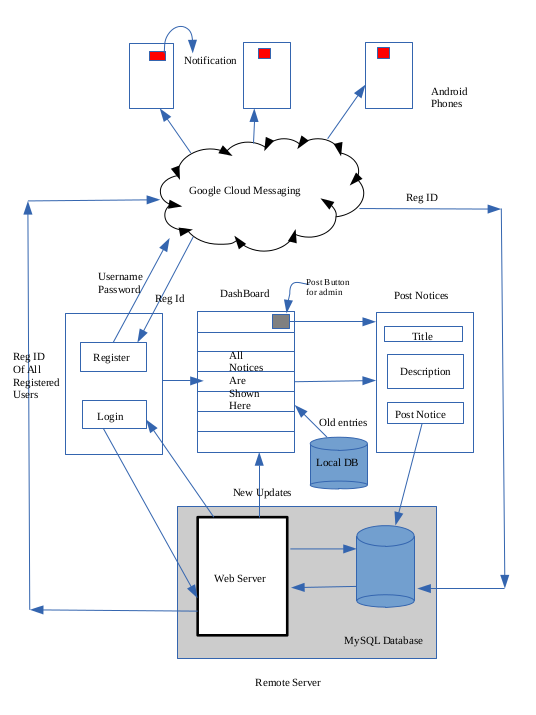
\includegraphics[scale=0.9]{image/detaildesign.png}
\caption{Detailed Design}
\end{figure}
\pagebreak

\section{System Design}
The system design can be clearly explained from the following diagrams:
\textbf{\emph{Use Case Diagram:}}\\

A Use Case diagram at its simplest is a representation of a user's interaction with the system and depicting the specifications of a use case. A use case diagram can portray the different types of users of a system and the various ways that they interact with the system. This type of diagram is typically used in conjunction with the textual use case and will often be accompanied by other types of diagrams as well.
\\
There are two types of user in this application, user and admin. Following depits their use case diagram:

\begin{figure}[H]
\centering 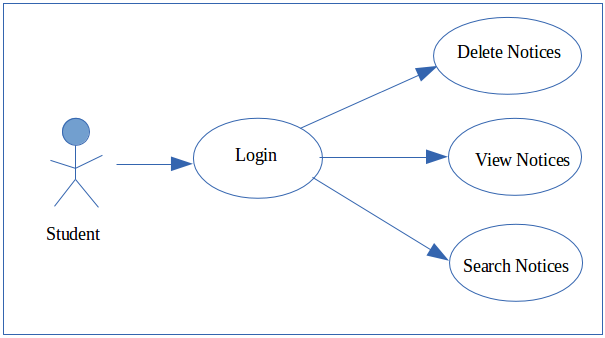
\includegraphics[scale=0.5]{image/usecase1.png}
\caption{Use Case Diagram For User}
\end{figure}

This diagram is showing what a normal user can do with this application. The user can login, after that he can view the notices, delete the notices and can search for particular notices.

\begin{figure}[H]
\centering 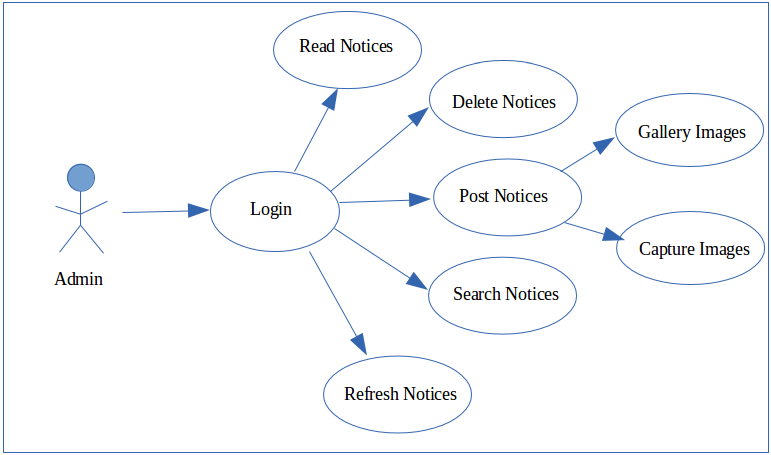
\includegraphics[scale=0.5]{image/usecase2.png}
\caption{Use Case Diagram For Admin}
\end{figure}

This diagram shows the priveleges of admin. An admin can post the notice in addition to viewing and deleting it. He can also post images as an attachment to the notices. Images can be choosen from the gallery or he can click the picture instantly usinng this application.






%%%%%%%%%%%%%%%%%%%%%%%%%%%%%%%%%%%%%%%%%%%%%%%%%%%%%%%%%%%%%%%%%%%%%%%%%%%%%%%%%%%%%%%%%%%%%%%%%%%%%%%%%%%%%%%%%%%%%%%%%%%%%%%%%
\pagebreak
\section{User Interface Design}
User Interface Design means the design of application with  which the user interacts. So it should be kept in mind that UI should be very simple and easy to use. It should be simple enough in look and feel also.
\begin{figure}[H]
\centering 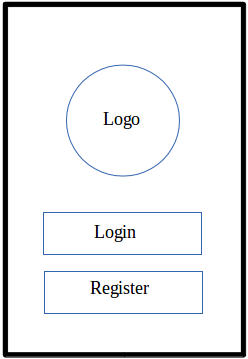
\includegraphics[scale=0.5]{image/ui1.png}
\caption{Landing Page}
\end{figure}

This page is the first page which is presented to the user. It has two buttons, to login or to register.

\begin{figure}[H]
\centering 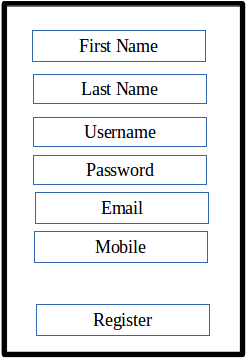
\includegraphics[scale=0.5]{image/ui2.png}
\caption{Registration Page}
\end{figure}

This is the registration page where the user get himself registered with the servers of this application.

\begin{figure}[H]
\centering 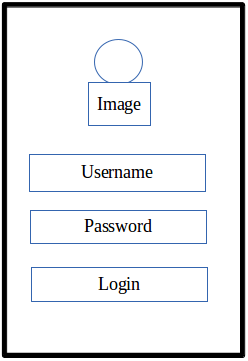
\includegraphics[scale=0.5]{image/ui3.png}
\caption{Login Page}
\end{figure}

This is the login page where user enters his username and password in order to access the notices.

\begin{figure}[H]
\centering 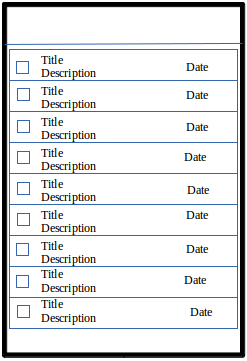
\includegraphics[scale=0.5]{image/ui4.png}
\caption{Dashboard Of Notices}
\end{figure}

This is the main dashboard, which receives all the notices from the user. The user can click on any notice, to see its details.
In addition to it, user can search and delete the notices.

\begin{figure}[H]
\centering 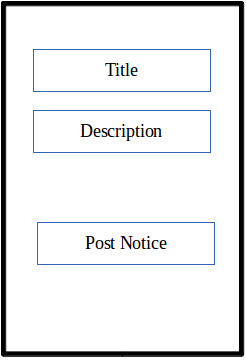
\includegraphics[scale=0.5]{image/ui5.png}
\caption{Post Notice Page}
\end{figure}

This page is only for the admin. Only admin can post the notices. He can choose images as attachment to notices.

\begin{figure}[H]
\centering 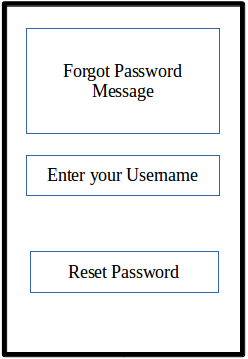
\includegraphics[scale=0.5]{image/ui6.png}
\caption{Reset Password Page}
\end{figure}

This is Reset Password page where the user can reset the password in order if he forgots his password.

%%%%%%%%%%%%%%%%%%%%%%%%%%%%%%%%%%%%%%%%%%%%%%%%%%%%%%%%%%%%%%%%%%%%%%%%%%%%%%%%%%%%%%%%%%%%%%%%%%%%%%%%%%%%%%%%%%%%%%%%%%%%%%
\pagebreak
\section{Database Design}
Database design is the process of producing a detailed data model of a database. This logical data model contains all the needed logical and physical design choices and physical storage parameters needed to generate a design in a data definition language, which can then be used to create a database. A fully attributed data model contains detailed attributes for each entity.\\

The term database design can be used to describe many different parts of the design of an overall database system. Principally, and most correctly, it can be thought of as the logical design of the base data structures used to store the data. In the relational model these are the tables and views. In an object database the entities and relationships map directly to object classes and named relationships. However, the term database design could also be used to apply to the overall process of designing, not just the base data structures, but also the forms and queries used as part of the overall database application within the database management system (DBMS).\\

The process of doing database design generally consists of a number of steps which will be carried out by the database designer. Usually, the designer must:
\begin{itemize}
\item Determine the relationships between the different data elements.
\item Superimpose a logical structure upon the data on the basis of these relationships.
\end{itemize}

\textbf{\emph{Design process}}
\begin{enumerate}

\item Determine the purpose of the database - This helps prepare for the remaining steps.
\item Find and organize the information required - Gather all of the types of information to record in the database, such as product name and order number.
\item Divide the information into tables - Divide information items into major entities or subjects, such as Products or Orders. Each subject then becomes a table.
\item Turn information items into columns - Decide what information needs to be stored in each table. Each item becomes a field, and is displayed as a column in the table. For example, an Employees table might include fields such as Last Name and Hire Date.
\item Specify primary keys - Choose each table’s primary key. The primary key is a column, or a set of columns, that is used to uniquely identify each row. An example might be Product ID or Order ID.
\item Set up the table relationships - Look at each table and decide how the data in one table is related to the data in other tables. Add fields to tables or create new tables to clarify the relationships, as necessary.
\item Refine the design - Analyze the design for errors. Create tables and add a few records of sample data. Check if results come from the tables as expected. Make adjustments to the design, as needed.
\item Apply the normalization rules - Apply the data normalization rules to see if tables are structured correctly. Make adjustments to the tables
\end{enumerate}

\subsection{ER Diagrams}
 An ER diagram is a diagram that helps to design databases in an efficient way.Attributes in ER diagrams are usually modeled as an oval with the name of the attribute, linked to the entity or relationship that contains the attribute.\\

Within the relational model the final step can generally be broken down into two further steps, that of determining the grouping of information within the system, generally determining what are the basic objects about which information is being stored, and then determining the relationships between these groups of information, or objects. \\

An Entity Relationship Diagram (ERD) is a visual representation of different data using conventions that describe how these data are related to each other. ER diagrams are most often associated with complex databases that are used in software engineering and IT networks. In particular, ER diagrams are frequently used during the design stage of a development process in order to identify different system elements and their relationships with each other. For example, an inventory software used in a retail shop will have a database that monitors elements such as purchases, item, item type, item source and item price.\\
The ER diagram of database used in the project is as follow:
\begin{figure}[H]
\centering 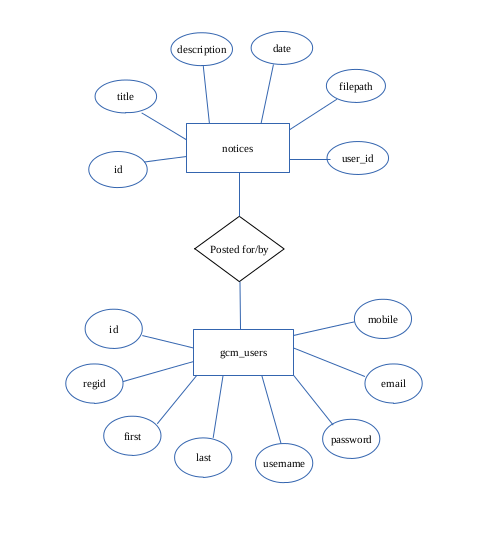
\includegraphics[scale=0.9]{image/erdiagram.png}
\caption{ER Diagram}
\end{figure}

\subsection{Normalization}
Normalization is a systematic way of ensuring that a database structure is suitable for general-purpose querying and free of certain undesirable characteristics—insertion, update, and deletion anomalies—that could lead to a loss of data integrity.
\\
A standard piece of database design guidance is that the designer should create a fully normalized design; selective denormalization can subsequently be performed, but only for performance reasons. However, some modeling disciplines, such as the dimensional modeling approach to data warehouse design, explicitly recommend non-normalized designs, i.e. designs that in large part do not adhere to 3NF. Normalization consists of normal forms that are 1NF, 2NF, 3NF, BOYCE-CODD NF (3.5NF), 4NF and 5NF.

\subsection{Database Manipulation}
Data Manipulation is retrieval of information from the database, insertion of new information into the database, deletion of information in the database modification of information in the database. A DML is a language which enables users to access and manipulate data.
The goal is to provide efficient human interaction with the system.\\

There are two types of DML:
\begin{enumerate}
\item \emph{Procedural:} In it, the user specifies what data is needed and how to get it.
\item \emph{Non Procedural:} In it, the user only specifies what data is needed. It is easier for user and may not generate code as efficient as that produced by procedural languages.
\end{enumerate}
 A query language is a portion of a DML involving information retrieval only. The terms DML and query language are often used synonymously. 
\subsection{Database Connection Control and Strings}
\begin{enumerate}
\item \textbf{\emph{Database connection control:}} It is a feature which prevents users from connecting to a database. This feature is also called passive shutdown because when connection control is invoked, users who are currently connected to the database remain unaffected until they disconnect. This capability is useful if you need to acquire exclusive access to a database to perform maintenance operations, such as compacting the database, or make updates to the database's design.\\

When connection control is invoked, users who are currently connected to a database remain unaffected until they disconnect from the database. At that point they will be unable to reconnect to the database until the user who invoked connection control revokes it or closes his or her connection to the database.\\

The following scenarios provide examples of how the connection control feature works. Assume there are five users in the database and that user five has invoked connection control on the database:\\

\textbf{Scenario 1} \\
User six tries to connect to the database, but is denied access, and an error message is returned stating that user five is preventing the database from being opened.

\textbf{Scenario 2} \\
User one closes the database and tries to reconnect to the database, but is denied access, and an error message is returned stating that user five is preventing the database from being opened.

\textbf{Scenario 3}\\
User five closes the database. User six tries to open the database and is successful. This is because connection control only persists while the user who invoked it remains connected to the database.

\textbf{Scenario 4}\\
Users one through four exit the database. User five uses the ADO OpenSchema method to retrieve a list of users in the database and determines that no other users are in the database. User five compacts the database, closes the database, and connection control is automatically revoked.

\item \textbf{\emph{Connection String:}} A connection string is a string that specifies information about a data source and the means of connecting to it. It is passed in code to an underlying driver or provider in order to initiate the connection. Whilst commonly used for a database connection, the data source could also be a spreadsheet or text file.

The connection string may include attributes such as the name of the driver, server and database, as well as security information such as user name and password.\\

\emph{Example of MySQL Connection String}\\
Server=myServerAddress;Port=1234;Database=myDataBase;Uid=myUsername;\\
Pwd=myPassword;\\

The port 3306 is the default MySql port. The value is ignored if Unix socket is used.
\end{enumerate}


%%%%%%%%%%%%%%%%%%%%%%%%%%%%%%%%%%%%%%%%%%%%%%%%%%%%%%%%%%%%%%%%%%%%%%%%%%%%%%%%%%%%%%%%%%%%%%%%%%%%%%%%%%%%%%%%%%%%%%%%%%%%%
\pagebreak
\section{Methodology}
The methodology used in project is Agile Software Development. Agile Software Development methodology is used especially for software development, that is characterized by the division of tasks into short phases of work and frequent reassessment and adaptation of plans.\\

It is for a project that needs extreme agility in requirements. The key features of agile are its short-termed delivery cycles (sprints), agile requirements, dynamic team culture, less restrictive project control and emphasis on real-time communication.\\

Agile software development is a group of software development methods based on iterative and incremental development, in which requirements and solutions evolve through collaboration between self-organizing, cross-functional teams. It promotes adaptive planning, evolutionary development and delivery, a time-boxed iterative approach, and encourages rapid and flexible response to change. It is a conceptual framework that promotes foreseen tight iterations throughout the development cycle.\\
\begin{figure}[H]
\centering 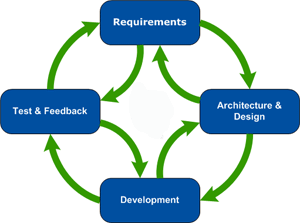
\includegraphics[scale=0.9]{image/agile.png}
\caption{Agile Software Development Methodology}
\end{figure}


The Manifesto of Agile Software Development context are:
\begin{itemize}
\item \emph{Individuals and interactions –} In agile development, self-organization and motivation are important, as are interactions like co-location and pair programming.
\item \emph{Working software –} Working software will be more useful and welcome than just presenting documents to clients in meetings.
\item \emph{Customer collaboration –} Requirements cannot be fully collected at the beginning of the software development cycle, therefore continuous customer or stakeholder involvement is very important.
\item \emph{Responding to change –} Agile development is focused on quick responses to change and continuous development.
\end{itemize}


%....................................
\chapter{Implementation,Testing and Maintenance}
\section{Introduction to Languages, IDE's,Tools and Technologies Used For Implementation}
\subsection{Java}
Java is a very popular
programming language developed by Sun Microsystems (now owned by
Oracle). Developed long after C and C++, Java incorporates many of the
powerful features of those powerful languages while addressing some of
their drawbacks. Still, programming languages are only as powerful as
their libraries. These libraries exist to help developers build applications.\\
Some of the Java’s important core features are:\\
\begin{itemize}
\item It’s easy to learn and understand.
\item It’s designed to be platform-independent and secure, using virtual machines.
\item It’s object-oriented.
\end{itemize}
Android relies heavily on these Java fundamentals. The Android SDK
includes many standard Java libraries (data structure libraries, mathlibraries, graphics libraries, networking libraries and everything else you could want) as well as special Android libraries that will help you develop awesome Android applications.\\
\textbf{\emph{Platform Independence Importance}}\\
With many programming languages, you need to use a compiler to reduce
your code down into machine language that the device can understand.
While this is well and good, different devices use different machine
languages. This means that you might need to compile your applications
for each different device or machine language—in other words, your code
isn’t very portable. This is not the case with Java. The Java compilers
convert your code from human readable Java source files to something
called “bytecode” in the Java world. These are interpreted by a Java
Virtual Machine, which operates much like a physical CPU might operate
on machine code, to actually execute the compiled code. Although it might
seem like this is inefficient, much effort has been put into making this
process very fast and efficient. These efforts have paid off in that Java
performance in generally second only to C/C++ in common language
performance comparisons.\\
Android applications run in a special virtual machine called the Dalvik
VM. While the details of this VM are unimportant to the average
developer, it can be helpful to think of the Dalvik VM as a bubble in which
your Android application runs, allowing you to not have to worry about
whether the device is a Motorola Droid, an HTC Evo, or the latest toaster
running Android. You don’t care so long as the device is Dalvik VM
friendly—and that’s the device manufacturer’s job to implement, not
yours.\\
\textbf{\emph{Why is Java Secure?}}\\
Let’s take this bubble idea a bit further. Because Java applications run
within the bubble that is a virtual machine, they are isolated from the
underlying device hardware. Therefore, a virtual machine can encapsulate,
contain, and manage code execution in a safe manner compared to
languages that operate in machine code directly. The Android platform
takes things a step further. Each Android application runs on the (Linux-
based) operating system using a different user account and in its own
instance of the Dalvik VM. Android applications are closely monitored by
the s.operating system and shut down if they don’t play nice (e.g. use toomuch processing power, become unresponsive, waste resources, etc.).\\
Therefore, it’s important to develop applications that are stable and
responsive. Applications can communicate with one another using well-
defined protocol.


\subsection{Android Development Tools}
\begin{itemize}
\item \textbf{\emph{Android SDK:}}\\
The Android Software Development Kit (Android SDK) contains the
necessary tools to create, compile and package Android applications. Most
of these tools are command line based. The primary way to develop
Android applications is based on the Java programming language.
\item \textbf{\emph{Android debug bridge (adb):}}\\
The Android SDK contains the Android debug bridge (adb), which is a
tool that allows you to connect to a virtual or real Android device, for the
purpose of managing the device or debugging your application.
\item \textbf{\emph{Android Developer Tools and Android Studio:}}\\
Google provides two integrated development environments (IDEs) to
develop new applications.The Android Developer Tools (ADT) are based on the Eclipse IDE. ADT
is a set of components (plug-ins), which extend the Eclipse IDE with
Android development capabilities.
Google also supports an IDE called Android Studio for creating Android
applications. This IDE is based on the IntelliJ IDE.\\
Both IDEs contain all required functionality to create, compile, debug and
deploy Android applications. They also allow the developer to create and
start virtual Android devices for testing.\\
Both tools provide specialized editors for Android specific files. Most of
Android's configuration files are based on XML. In this case these editors
allow you to switch between the XML representation of the file and a
structured user interface for entering the data.Dalvik Virtual Machine
The Android system uses a special virtual machine, i.e., the Dalvik Virtual
Machine (Dalvik) to run Java based applications. Dalvik uses a custom
bytecode format which is different from Java bytecode.
\\
Therefore you cannot run Java class files on Android directly; they need to
be converted into the Dalvik bytecode format.
\item \textbf{\emph{Android RunTime (ART):}}\\
With Android 4.4, Google introduced the Android RunTime (ART) as
optional runtime for Android 4.4. It is expected that versions after 4.4 will
use ART as default runtime. ART uses Ahead Of Time compilation. During the deployment process of
an application on an Android device, the application code is translated into
machine code. This results in approx. 30\% larger compile code, but allows
faster execution from the beginning of the application.

\end{itemize}

\subsection{Security and Permission Concept in Android}

\begin{itemize}
\item \textbf{\emph{Security Concept In Android:}}\\
The Android system installs every Android application with a unique user
and group ID. Each application file is private to this generated user, e.g.,
other applications cannot access these files. In addition each Android
application is started in its own process.\\

Therefore, by means of the underlying Linux kernel, every Android
application is isolated from other running applications.
If data should be shared, the application must do this explicitly via an
Android component which handles the sharing of the data, e.g., via a
service or a content provider.

\item \textbf{\emph{Permission concept in Android:}}\\
Android contains a permission system and predefines permissions for
certain tasks. Every application can request required permissions and also
define new permissions. For example, an application may declare that it
requires access to the Internet.\\

Permissions have different levels. Some permissions are automatically
granted by the Android system, some are automatically rejected. In most
cases the requested permissions are presented to the user before installing
the application. The user needs to decide if these permissions shall be
given to the application.\\

If the user denies a required permission, the related application cannot be
installed. The check of the permission is only performed during
installation, permissions cannot be denied or granted after the installation.\\

An Android application declares the required permissions in itsAndroidManifest.xml configuration file. It can also define additional
permissions which it can use to restrict access to certain components.
\end{itemize}


%%%%%%%%%%%%%%%%%%%%%%%%%%%%%%%%%%%%%%%%%%%%%%

\pagebreak
\section{Coding Standards of Language Used}
Coding Standards of Java are used in the whole project. This standard include the following:
\begin{itemize}
\item No wildcard imports.
\item Overloads appear sequentially.
\item Braces are used even when the body is empty or contains a single statement.
\item Two space indentation.
\item Column limit can be 80 or 100 characters.
\item No C-style array declarations.
\item Default statements required in switch statements.
\item Modifiers appear in the order recommended by the Java Language Specification.
\item Constants use CONSTANT\_CASE. Note that every constant is a static final field, but not all static final fields are constants.
\item Class name should start with uppercase letter.
\item Function name should start with lowercase letter.
\end{itemize}
%%%%%%%%%%%%%%%%%%%%%%%%%%%%%%%%%%%%%%%%%%%%%%%%%%%%
\pagebreak
\section{Project Scheduling}
Project scheduling is concerned with the techniques that can be employed to manage the activities that need to be undertaken during the development of a project. Scheduling is carried out in advance of the project commencing and involves:
\begin{itemize}
\item Identifying the tasks that need to be carried out.
\item Estimating how long they will take.
\item Allocating resources (mainly personnel).
\item Scheduling when the tasks will occur.
\end{itemize}
Once the project is underway control needs to be exerted to ensure that the plan continues to represent the best prediction of what will occur in the future based on what occurs during the development and often necessitates revision of the plan.
Effective project planning will help to ensure that the systems are delivered:
\begin{itemize}
\item Within cost;
\item Within the time constraint;
\item To a specific standard of quality.
\end{itemize}

Two project scheduling techniques will be presented, the Milestone Chart and Gantt Chart.
\begin{enumerate}
\item \textbf{\emph{Milestone Charts:}}\\
Milestones mark significant events in the life of a project, usually critical activities which must be achieved on time to avoid delay in the project. Milestones should be truely significant and be reasonable in terms of deadlines (avoid using intermediate stages).
\\
Examples include:
\begin{itemize}
\item Installation of equipment.
\item Completion of phases.
\item File conversion.
\item Cut over to the new system
\end{itemize}

\item \textbf{\emph{Gantt Charts:}}\\
A Gantt chart is a horizontal bar or line chart which will commonly include the following features:
\begin{itemize}
\item Activities identified on the left hand side.
\item Time scale is drawn on the top (or bottom) of the chart.
\item A horizontal open oblong or a line is drawn against each activity indicating estimated duration.
\item Dependencies between activities are shown.
\item At a review point the oblongs are shaded to represent the actual time spent (an alternative is to represent actual and estimated by 2 separate lines).
\item A vertical cursor (such as a transparent ruler) placed at the review point makes it possible to establish activities which are behind or ahead of schedule.
\end{itemize}
\end{enumerate}

Following is the chart of various commits on github, while developing this application:
\begin{figure}[H]
\centering 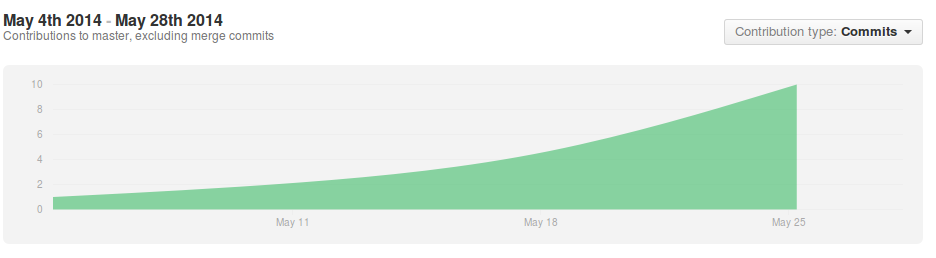
\includegraphics[scale=0.4]{image/commit.png}
\caption{Graph of Commits on GitHub}
\end{figure}
This graph is showing commit in last week of May. It depicts how many times, changes are pushed on to githu after testing.
\begin{figure}[H]
\centering 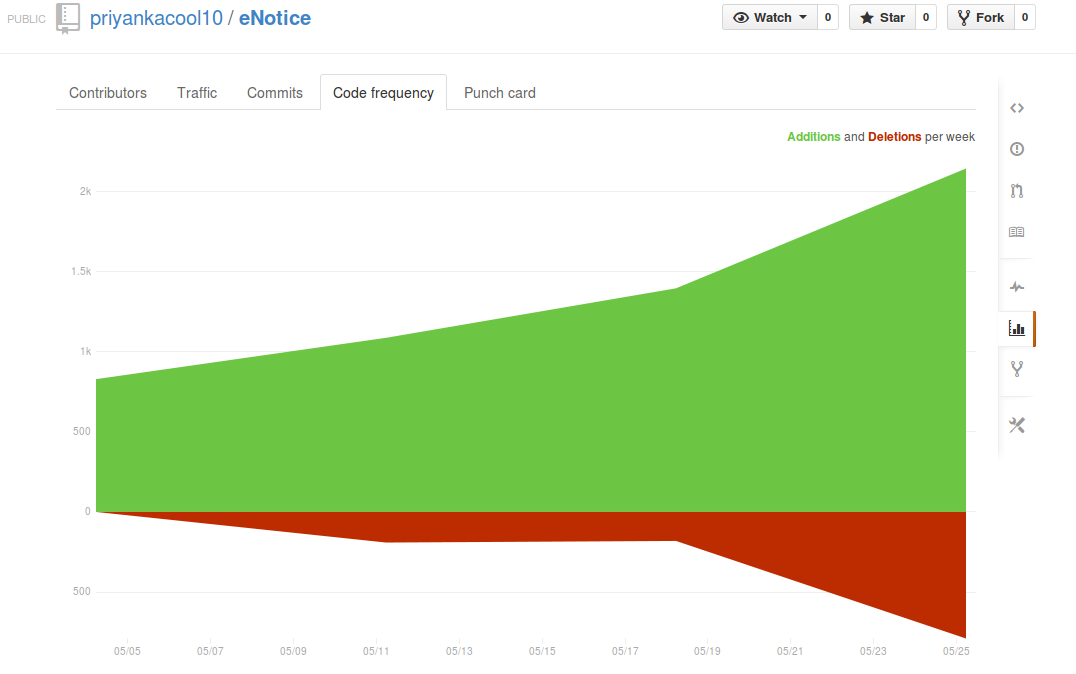
\includegraphics[scale=0.4]{image/codefrequency.png}
\caption{Code Frequency Graph on GitHub}
\end{figure}
This graph depicts the frequency of code that is pushed on github on respective dates.

%%%%%%%%%%%%%%%%%%%%%%%%%%%%%%%%%%%%%%%%%%%%%%%%%%%%%%%%%%%
\pagebreak
\section{Test Plan and Test Activities}
\subsection{Test Plan}
A test plan can be defined as a document describing the scope, approach, resources, and schedule of intended testing activities. It identifies test items, the features to be tested, the testing tasks, who will do each task, and any risks requiring contingency planning.
In software testing, a test plan gives detailed testing information regarding an upcoming testing effort, including\\
\begin{itemize}
\item Scope of testing
\item Schedule
\item Test Deliverables
\item Release Criteria
\item Risks and Contingencies 
\end{itemize}
It is also be described as a detail of how the testing will proceed, who will do the testing, what will be tested, in how much time the test will take place, and to what quality level the test will be performed.\\

The process of defining a test project so that it can be properly measured and controlled. The test planning process generates a high level test plan document that identifies the software items to be tested, the degree of tester independence, the test environment, the test case design and test measurement techniques to be used, and the rationale for their choice.\\

A testing plan is a methodological and systematic approach to testing a system such as a machine or software. It can be effective in finding errors and flaws in a system. In order to find relevant results, the plan typically contains experiments with a range of operations and values, including an understanding of what the eventual workflow will be.\\

Test plan is a document which includes, introduction, assumptions, list of test cases, list of features to be tested, approach, deliverables, resources, risks and scheduling. A test plan is a systematic approach to testing a system such as a machine or software. The plan typically contains a detailed understanding of what the eventual workflow will be.
A record of the test planning process detailing the degree of tester indedendence, the test environment, the test case design techniques and test measurement techniques to be used, and the rationale for their choice.

\subsection{Test Activities}
Various Testing Activities are as follow:
\begin{enumerate}
\item \textbf{\emph{Black box testing –}} Internal system design is not considered in this type of testing. Tests are based on requirements and functionality.

\item \textbf{\emph{White box testing –}} This testing is based on knowledge of the internal logic of an application’s code. Also known as Glass box Testing. Internal software and code working should be known for this type of testing. Tests are based on coverage of code statements, branches, paths, conditions.

\item \textbf{\emph{Unit testing –}} Testing of individual software components or modules. Typically done by the programmer and not by testers, as it requires detailed knowledge of the internal program design and code. may require developing test driver modules or test harnesses.

\item \textbf{\emph{Incremental integration testing –}} Bottom up approach for testing i.e continuous testing of an application as new functionality is added; Application functionality and modules should be independent enough to test separately. done by programmers or by testers.

\item \textbf{\emph{Integration testing –}} Testing of integrated modules to verify combined functionality after integration. Modules are typically code modules, individual applications, client and server applications on a network, etc. This type of testing is especially relevant to client/server and distributed systems.

\item \textbf{\emph{Functional testing –}} This type of testing ignores the internal parts and focus on the output is as per requirement or not. Black-box type testing geared to functional requirements of an application.

\item \textbf{\emph{System testing –}} Entire system is tested as per the requirements. Black-box type testing that is based on overall requirements specifications, covers all combined parts of a system.

\item \textbf{\emph{End-to-end testing –}} Similar to system testing, involves testing of a complete application environment in a situation that mimics real-world use, such as interacting with a database, using network communications, or interacting with other hardware, applications, or systems if appropriate.

\item \textbf{\emph{Acceptance testing -}} Normally this type of testing is done to verify if system meets the customer specified requirements. User or customer do this testing to determine whether to accept application.

\item \textbf{\emph{Usability testing –}} User-friendliness check. Application flow is tested, Can new user understand the application easily, Proper help documented whenever user stuck at any point. Basically system navigation is checked in this testing.
\end{enumerate}

%..................
\chapter{Results and Discussions}
\section{User Interface Representation}
In order to make user interface, many controls are used. Some of which are as follow:
\begin{enumerate}
\item \textbf{\emph{TextView:}}\\
Text View displays text to the user and optionally allows them to edit it. A TextView is a complete text editor, however the basic class is configured to not allow editing.

\item \textbf{\emph{EditText:}}\\
EditText is a thin veneer over TextView that configures itself to be editable. 
\item \textbf{\emph{Button:}}\\
A button consists of text or an icon (or both text and an icon) that communicates what action occurs when the user touches it.

\item \textbf{\emph{List View:}}\\
ListView is a view group that displays a list of scrollable items. The list items are automatically inserted to the list using an Adapter that pulls content from a source such as an array or database query and converts each item result into a view that's placed into the list.

\item \textbf{\emph{Check Boxes:}}\\
Checkbox is a control or widget that can be activated with a finger touch and can be polled in the application's code for
a checked and uncheckked state.

\end{enumerate}
\subsection{Brief Description of Various Modules}
\subsubsection{GCM Messaging}
Google Cloud Messaging for Android (GCM) is a service that allows you to send data from your server to your users' Android-powered device, and also to receive messages from devices on the same connection. The GCM service handles all aspects of queueing of messages and delivery to the target Android application running on the target device. GCM is completely free no matter how big your messaging needs are, and there are no quotas.

\textbf{\emph{GCM Working}}
\begin{enumerate}
\item Android device sends SENDER\_ID to GCM Server for registration.
\item After successful registration, GCM sends Registration ID to Android device.
\item After getting registration id, Android device sends registration id to Web Server.
\item Store registration id in our database at the server.
\item Whenever Push Notification needed, get registration ids from server, and send the request to GCM with registration id and message.
\item After push notification request, GCM sends Push Notifications to Android device.
\end{enumerate}

\begin{figure}[H]
\centering 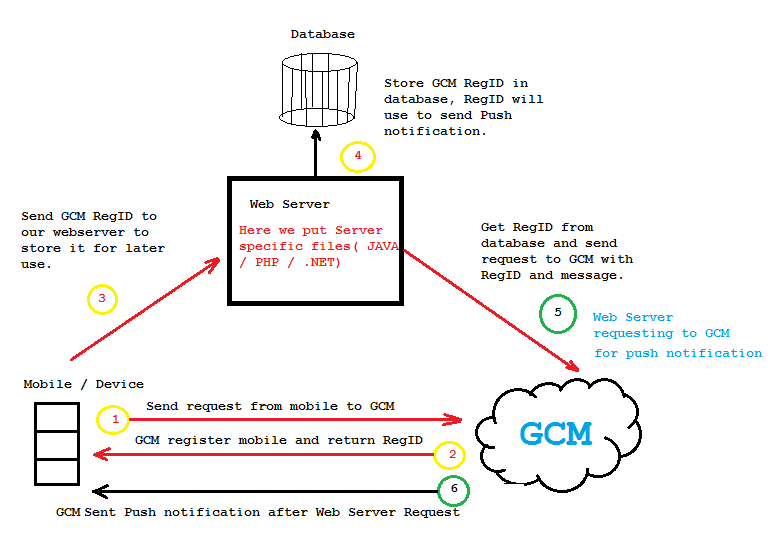
\includegraphics[scale=0.5]{image/gcm.png}
\caption{Google Cloud Messaging Working}
\end{figure}
Following are the steps to use GCM in android project:
\begin{enumerate}
\item Register with Google Cloud Messaging from GOOGLE API Console and get Sender ID and API key for Google Cloud Messaging.
\item Set Emulator for Google Cloud Messaging helper library.
\item Create Android project to register with Google Cloud Messaging(GCM).
\item Create server side code to save Google Cloud Messaging registration id in our database and send push notification to device.
\end{enumerate}

\subsubsection{HTTP Connections To Web Server}
Steps to have HTTP connection to Web Server are as follow:
\begin{enumerate}
\item Declare Internet permissions in the manifest by adding the following line to AndroidManifest.xml.
\item Create your HttpClient and HttpPost objects to execute the POST request. 
\item Set your POST data. This is done by creating and setting a list of NameValuePairs as your HttpPost's entity. Be sure to catch the UnsupportedEncodingException thrown by HttpPost.setEntity().
\item Execute the POST request. This returns an HttpResponse object, whose data can be extracted and parsed. Be sure to catch the ClientProtocolException and IOException thrown.
\end{enumerate}

\subsubsection{JSON Parsing}
JSON stands for JavaScript Object Notation.It is an independent data exchange format and is the best alternative for XML.
Steps of JSON Parsing are:
\begin{enumerate}
\item For parsing a JSON object, we will create an object of class JSONObject and specify a string containing JSON data to it. 
\item An JSON file consist of different object with different key/value pair e.t.c. So JSONObject has a seperate function for parsing each of the component of JSON file.
\end{enumerate}

\subsubsection{Broadcast Receiver}
Broadcast receiver is a component that responds to system conditions such as low battery or the screen being turned off. You can
use broadcast receivers to initiate a response from a running application, such as if a picture has been taken.
\subsubsection{Services}
Service is a process that runs in background to perform long term operations or work for remote processes. Services don't provide a User Interface.

\subsubsection{Content Provider}
It manages persistent data on the device or external sources such as web or cloud or any other system application has access to.
Android devices has on-board SQLite database management system to provide organized persistent data storage.
%%%%%%%%%%%%%%%%%%%%%%%%%%%%%%%%%%%%%%%%%%%%%%%%%%%%%%%%%%%%%%%%%
\pagebreak
\section{SnapShots of System}
Following are the snapshots of working application:
\begin{figure}[H]
\centering 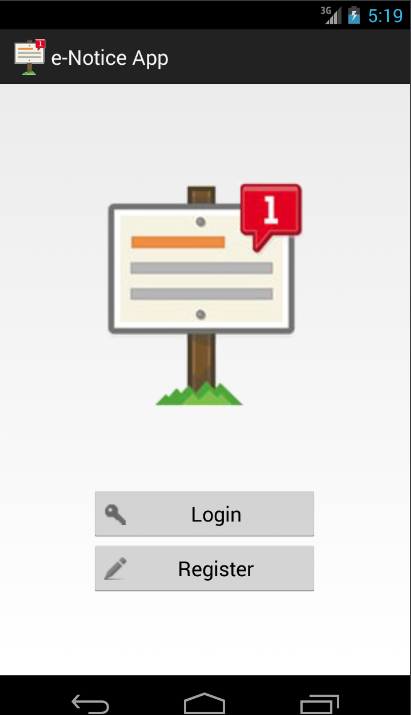
\includegraphics[scale=0.7]{image/landing.png}
\caption{Landing Page}
\end{figure}
This is the first page, the user is presented with at the first time, when he opens the application.

\begin{figure}[H]
\centering 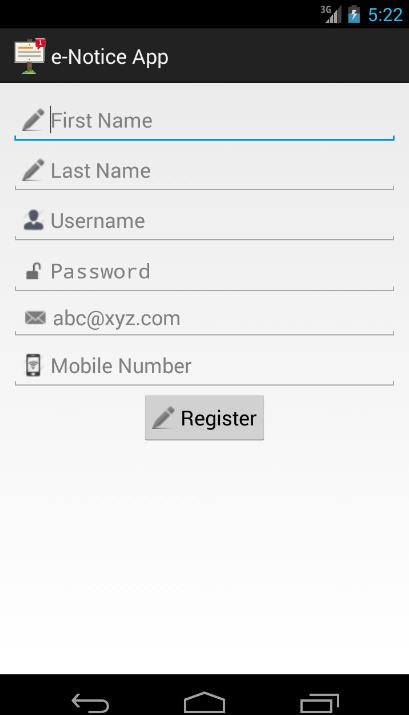
\includegraphics[scale=0.7]{image/register.png}
\caption{Register Page}
\end{figure}
This is the page where user registers himself to GCM and Web Server.

\begin{figure}[H]
\centering 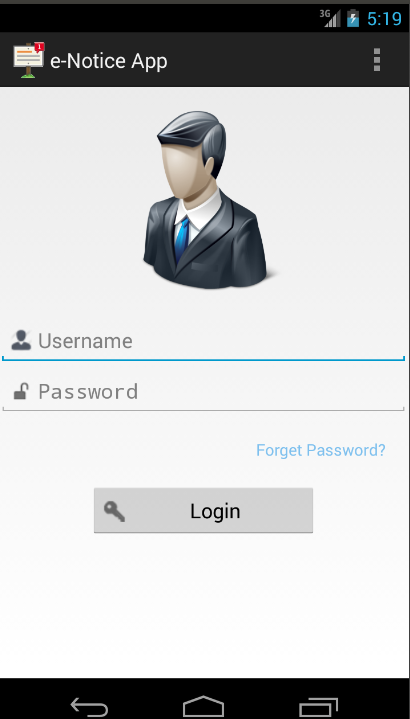
\includegraphics[scale=0.7]{image/login.png}
\caption{Login Page}
\end{figure}
This page is used to login to the application.

\begin{figure}[H]
\centering 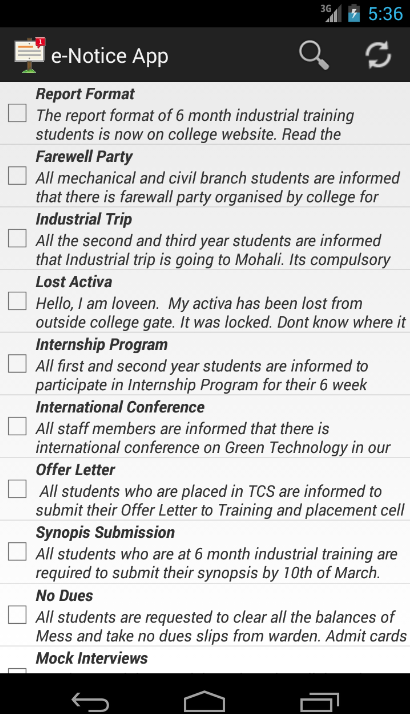
\includegraphics[scale=0.7]{image/dashboard.png}
\caption{DashBoard Page}
\end{figure}

In this page, all the notices are displayed. This is the main panel that is requierd by the normal user of application.
The user will tap on a particular notice in order to view details of notices.

\begin{figure}[H]
\centering 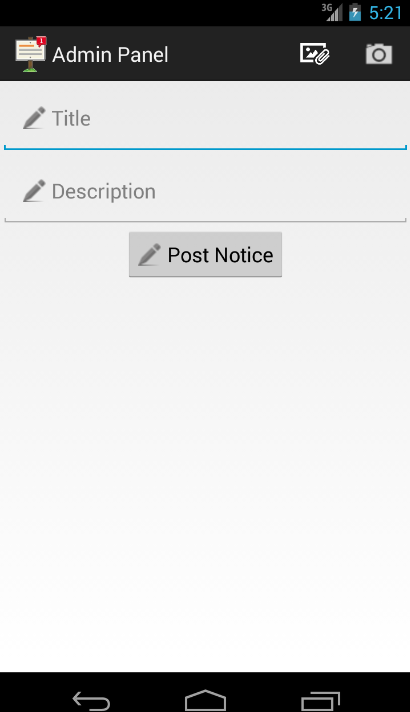
\includegraphics[scale=0.7]{image/post.png}
\caption{Post Notices Page}
\end{figure}
This is an Admin Panel Page where admin is allowed to post the message. Admin has two options of attaching image to notice.
First is to pick up image from gallery and second is to take an image from camera instantly and post with the notice.

\begin{figure}[H]
\centering 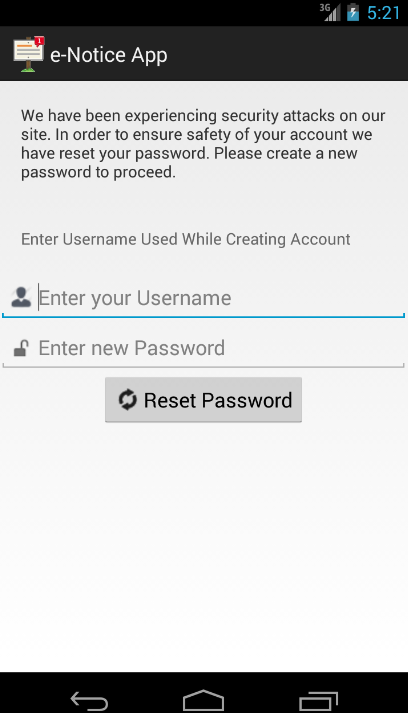
\includegraphics[scale=0.7]{image/reset.png}
\caption{Reset Password Page}
\end{figure}

This page is presented to the user when user forgots his password and want to reset the password.

\begin{figure}[H]
\centering 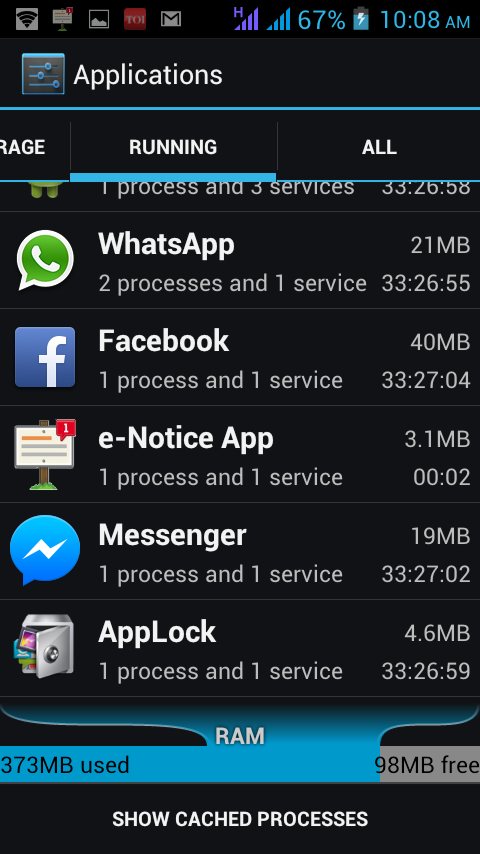
\includegraphics[scale=0.7]{image/service.png}
\caption{Intent Service Running In Application}
\end{figure}

This figure shows that service of application starts running, whenever any GCM notification arrives.

\begin{figure}[H]
\centering 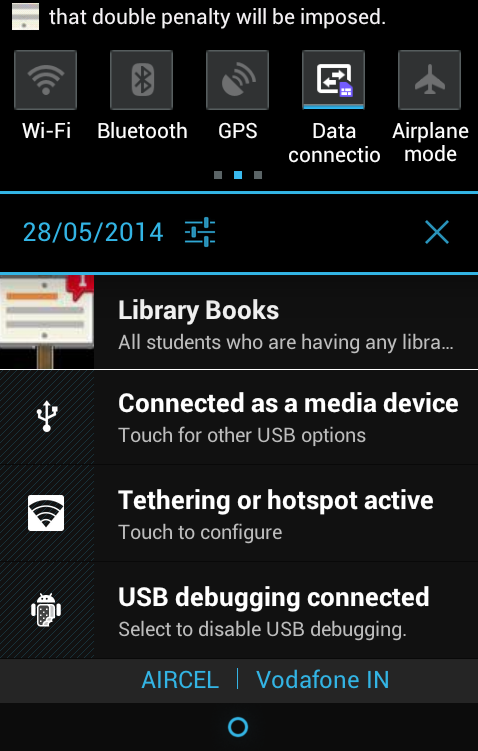
\includegraphics[scale=0.7]{image/notify.png}
\caption{Notification Received}
\end{figure}

This figure shows the notification received by the user from GCM server, whenever any notice is posted by the admin.

\begin{figure}[H]
\centering 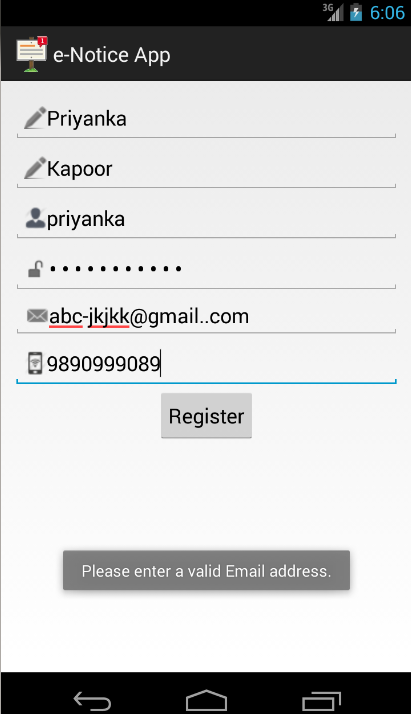
\includegraphics[scale=0.7]{image/email.png}
\caption{Email Validation}
\end{figure}

This figure shows the email validations implemented inside the application.

\begin{figure}[H]
\centering 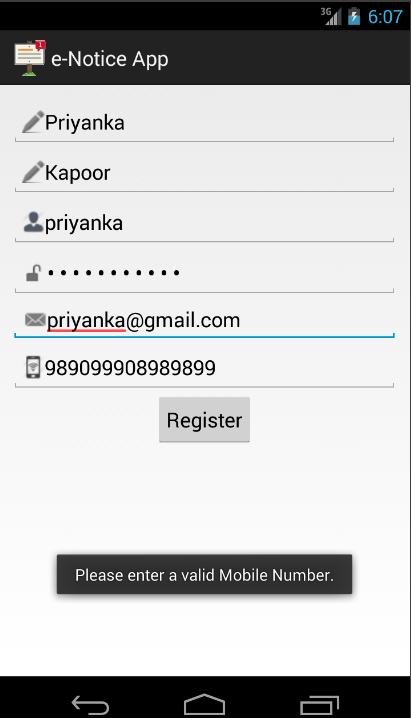
\includegraphics[scale=0.7]{image/mob.png}
\caption{Mobile Number Validation}
\end{figure}
This figure shows the mobile number validation implemented in the application.

\begin{figure}[H]
\centering 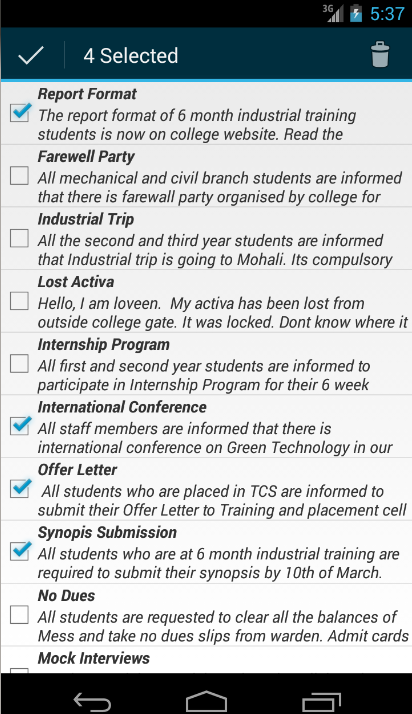
\includegraphics[scale=0.7]{image/context.png}
\caption{Contextual Action Bar}
\end{figure}
Contextual Action bar is implemented with the help of which, user is able to delete the notice.

\begin{figure}[H]
\centering 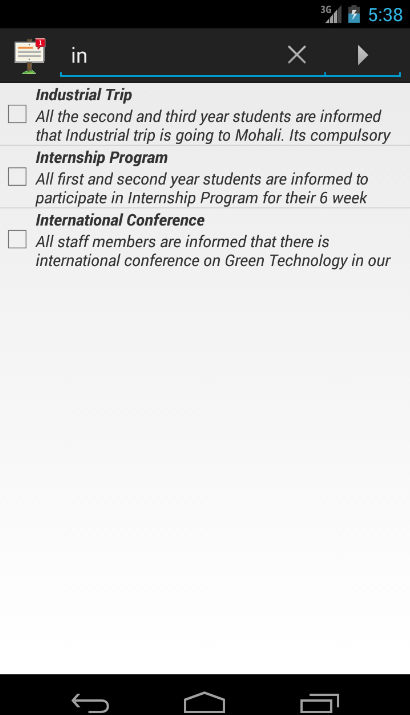
\includegraphics[scale=0.7]{image/search.png}
\caption{Search Box}
\end{figure}

This figure shows the search box available for the ease of user to search any notice by its title.

\begin{figure}[H]
\centering 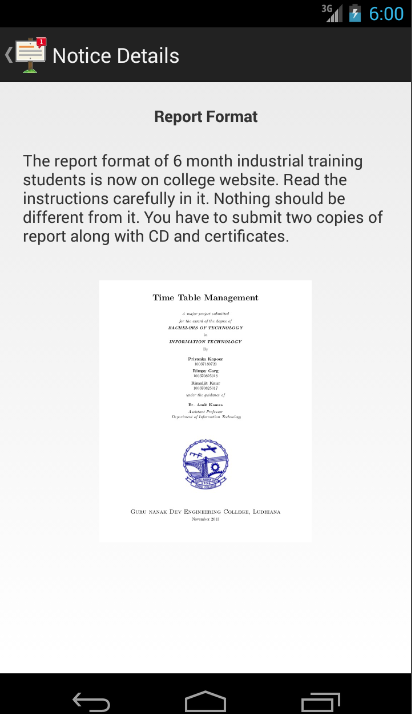
\includegraphics[scale=0.7]{image/detail.png}
\caption{Notice Details}
\end{figure}

This figure is showing the details of a particular notice that is tapped by the user.
%%%%%%%%%%%%%%%%%%%%%%%%%%%%%%%%%%%%%%%%%%%%%%%%%%%%%%%%%%%%%%%%%%%%%%%%%%%%%%%%%%%%%%%%%%%%%%%%%%%%%%%%%%%%%%%%%%%%%%%%%%%%%%%
\pagebreak
\section{Back End Representations}
The database used at the Back-end is MySQL database. Web Server used is Apache. Server side scripting language used is PHP.

Database design used at backend server has the following tables:

\begin{figure}[H]
\centering 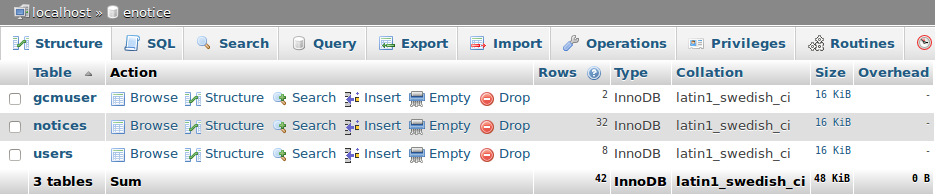
\includegraphics[scale=0.5]{image/db.png}
\caption{Tables inside Database}
\end{figure}

The first table is "gcmuser" which contains registration id given by GCM along with all personal information of the user.
The second table is "user" which just contains the id, username and password of the user.
The third table is "notices". It contains notice id, title and description of the notice, date on which the notice is posted
and filepath if a notice has an attachment.

\subsection{Snapshots of Database Tables}

\begin{figure}[H]
\centering 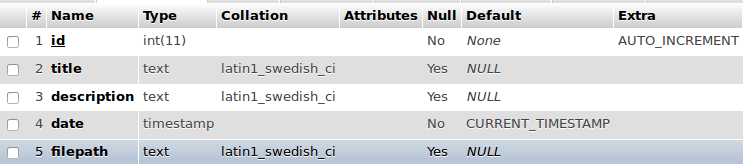
\includegraphics[scale=0.5]{image/db1.png}
\caption{Schema of GCM User Table}
\end{figure}
This table contains registration id given by GCM along with all personal information of the user like first name, last name, email id and
phone number.

\begin{figure}[H]
\centering 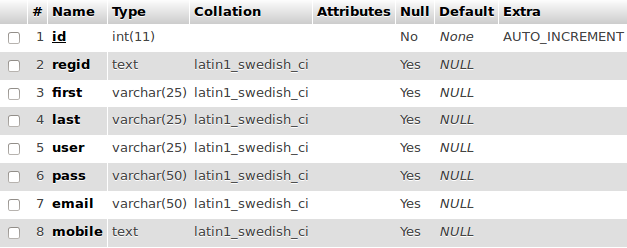
\includegraphics[scale=0.5]{image/db2.png}
\caption{Schema of User Table}
\end{figure}
This table just contains the id, username and password of the user.


\begin{figure}[H]
\centering 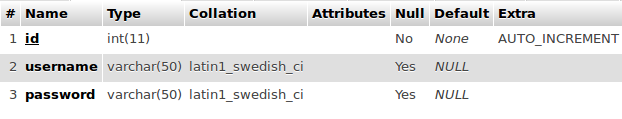
\includegraphics[scale=0.5]{image/db3.png}
\caption{Schema of Notices Table}
\end{figure}
This table contain all the details about the notices like notice id, title, description, date of notice post and filepath if the notice has an attachment.

\chapter{Conclusion and Future Scope}
\section{Future Scope}
The future scope of the project is that it can be used as any news giving application or it can be used to advertise your products,
telling the customers about new schemes and products coming to your shop.
This application of e-Notice can be further extended to include the following features:
\begin{enumerate}
\item \textbf{\emph{Categorization of Notice:}}\\
Notices can be categorized in different categories, so that its possible for user to easily manage the notices.
Categorisation can also be done by making groups. Defining the notice to be circulated in a particular group can make it more secure.

\item \textbf{\emph{Documents and PDF files:}}\\
The attachments can be further improved to include PDF files or Doc files. Then there will not be much need to send images with the notices.
A single file would serve all the purposes.

\item \textbf{\emph{Feedback:}}\\
Feedback on the notices can also be taken. It can increase communication among connected members and any issue can be easily sorted out on the spot.
\end{enumerate}
%%%%%%%%%%%%%%%%%%%%%%%%%%%%%%%%%%%%%%%%%%%%%%%%%%%%%%%%%%%%%%%%%%%%%%%%%%%%%%%%%%%%%%%%%
\pagebreak
\section{Conclusion}

I learned a lot by doing this project.
\begin{itemize}
\item Operating system:
Ubuntu
\item Languages used:
Java, Android UI, PHP for backend
\item Servers Used:
LAMP Server, GCM Server
\item Database:
MySQL, SQLite
\item Typesetting by:
\LaTeX
\end{itemize}
So during this project I learned all the above things. Before this project, I had no idea about
Java and Android for making application. Although I had little bit knowledge of
Ubuntu before. But now I learned a lot about Ubuntu and got knowledge of using Android and Java for developing mobile
application and PHP for server side scripting. Now I prefer to work on command line rather than graphically. I learned how to work
on shell script.\\
If I talk about the project, e-Notice Application has reduced lot of manual work. It has made notififying each and every user very easy and taht too with no time and place restrictions.


                               %% More section can be added as per requirement


%-------------------------------------------------------------
 %\addto\captionsenglish{\renewcommand{\refname}{References}}
%% Here example is given for  writing a  bibliography

\renewcommand{\bibname}{References}

\begin{thebibliography}{9}

\bibitem{Android Tutorials}
Basic Android Tutorials, available at \url{http://www.tutorialspoint.com/android}

\bibitem{Android Developer Tutorials}
Android Development Tutorials, available at \url{http://www.developer.android.com}

\bibitem{Android Book}
Android Book. Wei-Meng Lee, \emph{Android 4 Application Development}, John Wiley \& Sons, Inc., 2012

\bibitem{Wikipedia}
\LaTeX Book. Donald E. Knuth, The \emph{TeXbook}, Addison–Wesley, Boston, 1986

\end{thebibliography}
 		%Referrences
%------------------------------------------------------------------------


\end{document}
%%------------------------End document-------------------------%%
